\setcounter{definition}{0} \setcounter{property}{0} \setcounter{claim}{0} \setcounter{fact}{0} \setcounter{corollary}{0} \setcounter{figure}{0}
\section{Dijkstra's Algorithm}


We now study the single-source shortest path problem with positive edge length:
given graph $G = (V, E)$ with edge length $l(e) > 0$ for any $e\in E$ and
source vertex $s\in V$, to seek $distance(s, v)$ for any $v\in V$.
We solve this problem with the \emph{Dijkstra's algorithm}.

Similar to BFS, the idea of Dijkstra's algorithm is also to
determine and calculate the distance of each vertex
in increasing order of distance.
More specifically, let $R = (v_1^*, v_2^*, \cdots, v_n^*)$, $n = |V|$,
be the order of vertices with increasing distance, i.e., $distance(s, v_k^*) \le distance(s, v_{k+1}^*)$, $1\le k < n$.
In other words, we define $v_k^*$ as the $k$-th closest vertex from $s$.
We don't know this order in advance.
But Dijktra's algorithm will identify vertices in this order and calculate
their distance.
For the sake of writing and notations, we define $R_k = \{v_1^*, v_2^*, \cdots, v_k^*\}$, i.e., 
the first $k$ vertices in above list; $R_k$ are also the closest $k$ vertices from $s$.

Clearly, $v_1^* = s$, $distance(s, v_1^*) = distance(s, s) = 0$, and $R_1 = \{s\}$.
The key question is: given $R_k$~(i.e., the closest $k$ vertices from $s$) and their distances~(i.e., $distance(s, v)$ for every $v\in R_k$),
how to find $v_{k + 1}^*$?
Below we show that $v_{k + 1}^*$ must be within \emph{one-edge extension} of $R_k$.
\begin{claim}
There must exist vertex $u\in R_k$ such that $(u, v_{k+1}^*) \in E$.
\end{claim}
\emph{Proof.} Suppose conversely that for every $u\in R_k$ we have $(u, v_{k+1}^k)\not\in E$.
Consider the shortest path from $s$ to $v_{k+1}^*$.
Let $w$ be the vertex right before $v_{k+1}^*$ in path $p$, i.e, $(w, v_{k+1}^*)$ is the last edge of $p$.
We have $distance(s, v_{k+1}^*) = distance(s, w) + l(w, v_{k+1}^*)$. %following the optimal substructure property.
As edges have positive edge length, we have $l(w, v_{k+1}^*) > 0$, and consequently
$distance(s, w) < distance(s, v_{k+1}^*)$.
Besides, according to the assumption, we have $w\not\in R_k$.
Therefore, $v_{k+1}^*$ cannot be the $(k+1)$-th closest vertex from $s$,
because $w$ has a shorter distance than $v_{k+1}^*$. This contradicts to the definition of $v_{k+1}^*$.\qed

Note that, in above proof, we use the fact that edges have positive lengths.
Hence, above claim may not be true for graphs with negative edge length.
This also explains why Dijkstra's algorithm does not work for graphs with negative edge length.


The above claim shows that, the last edge $(u,v)$ of the shortest path from $s$ to $v_{k+1}^*$
satisfies that $u\in R_k$ and $v\not\in R_k$. Which such edge is the correct one?
We don't know, so we enumerate all such edges $(u,v)\in E$ with $u\in R_k$ and $v\not\in R_k$.
Suppose that $(u,v)$ is the last edge of the shortest path from $s$ to $v_{k+1}^*$,
%then following the optimal substructure property,
we know that $distance(s,v) = distance(s,u) + l(u,v)$.
This leads to the following formula to calculate $v_{k+1}^*$ and its predecessor in the shortest path.
See an example in Figure~\ref{fig:extension}.

\begin{figure}[!h]
\centering{

\tikzset{every picture/.style={line width=0.75pt}} %set default line width to 0.75pt        

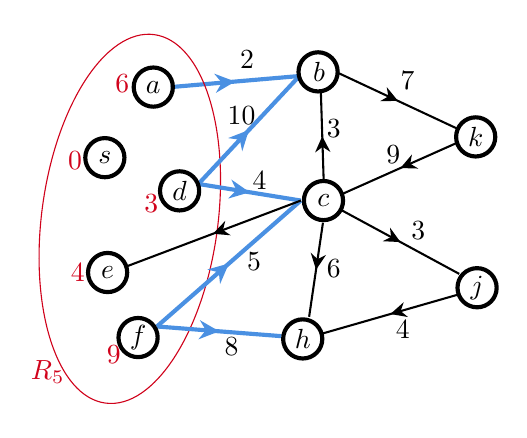
\begin{tikzpicture}[x=0.5pt,y=0.5pt,yscale=-1,xscale=1]
%uncomment if require: \path (0,296); %set diagram left start at 0, and has height of 296

%Straight Lines [id:da3320252336737717] 
\draw [color={rgb, 255:red, 74; green, 144; blue, 226 }  ,draw opacity=1 ][line width=1.5]    (119,48) -- (212,40) ;
\draw [shift={(165.5,44)}, rotate = 535.0799999999999] [fill={rgb, 255:red, 74; green, 144; blue, 226 }  ,fill opacity=1 ][line width=0.08]  [draw opacity=0] (14.56,-6.99) -- (0,0) -- (14.56,6.99) -- (9.67,0) -- cycle    ;
%Shape: Ellipse [id:dp2857420369455096] 
\draw  [color={rgb, 255:red, 208; green, 2; blue, 27 }  ,draw opacity=1 ] (26.24,134.88) .. controls (35.95,61.34) and (72.1,5.46) .. (106.98,10.07) .. controls (141.87,14.67) and (162.28,78.02) .. (152.57,151.56) .. controls (142.86,225.1) and (106.71,280.98) .. (71.83,276.37) .. controls (36.94,271.77) and (16.53,208.42) .. (26.24,134.88) -- cycle ;
%Straight Lines [id:da02943457575339692] 
\draw [color={rgb, 255:red, 74; green, 144; blue, 226 }  ,draw opacity=1 ][line width=1.5]    (139,118) -- (212,40) ;
\draw [shift={(175.5,79)}, rotate = 493.1] [fill={rgb, 255:red, 74; green, 144; blue, 226 }  ,fill opacity=1 ][line width=0.08]  [draw opacity=0] (14.56,-6.99) -- (0,0) -- (14.56,6.99) -- (9.67,0) -- cycle    ;
%Straight Lines [id:da7032022658079198] 
\draw [color={rgb, 255:red, 74; green, 144; blue, 226 }  ,draw opacity=1 ][line width=1.5]    (139,118) -- (213,130) ;
\draw [shift={(176,124)}, rotate = 189.21] [fill={rgb, 255:red, 74; green, 144; blue, 226 }  ,fill opacity=1 ][line width=0.08]  [draw opacity=0] (14.56,-6.99) -- (0,0) -- (14.56,6.99) -- (9.67,0) -- cycle    ;
%Straight Lines [id:da9416797747261806] 
\draw [color={rgb, 255:red, 74; green, 144; blue, 226 }  ,draw opacity=1 ][line width=1.5]    (109,221) -- (213,130) ;
\draw [shift={(161,175.5)}, rotate = 498.81] [fill={rgb, 255:red, 74; green, 144; blue, 226 }  ,fill opacity=1 ][line width=0.08]  [draw opacity=0] (14.56,-6.99) -- (0,0) -- (14.56,6.99) -- (9.67,0) -- cycle    ;
%Straight Lines [id:da6197316893700862] 
\draw [color={rgb, 255:red, 74; green, 144; blue, 226 }  ,draw opacity=1 ][line width=1.5]    (109,221) -- (199,228) ;
\draw [shift={(154,224.5)}, rotate = 184.45] [fill={rgb, 255:red, 74; green, 144; blue, 226 }  ,fill opacity=1 ][line width=0.08]  [draw opacity=0] (14.56,-6.99) -- (0,0) -- (14.56,6.99) -- (9.67,0) -- cycle    ;
%Straight Lines [id:da7705917014251779] 
\draw [color={rgb, 255:red, 0; green, 0; blue, 0 }  ,draw opacity=1 ][line width=0.75]    (86,178) -- (213,130) ;
\draw [shift={(149.5,154)}, rotate = 339.3] [fill={rgb, 255:red, 0; green, 0; blue, 0 }  ,fill opacity=1 ][line width=0.08]  [draw opacity=0] (11.61,-5.58) -- (0,0) -- (11.61,5.58) -- (7.71,0) -- cycle    ;
%Straight Lines [id:da7178806242260687] 
\draw [color={rgb, 255:red, 0; green, 0; blue, 0 }  ,draw opacity=1 ][line width=0.75]    (326,78) -- (240.5,38) ;
\draw [shift={(283.25,58)}, rotate = 205.07] [fill={rgb, 255:red, 0; green, 0; blue, 0 }  ,fill opacity=1 ][line width=0.08]  [draw opacity=0] (11.61,-5.58) -- (0,0) -- (11.61,5.58) -- (7.71,0) -- cycle    ;
%Straight Lines [id:da2873203830948724] 
\draw [color={rgb, 255:red, 0; green, 0; blue, 0 }  ,draw opacity=1 ][line width=0.75]    (326.5,88) -- (243.5,125) ;
\draw [shift={(285,106.5)}, rotate = 335.97] [fill={rgb, 255:red, 0; green, 0; blue, 0 }  ,fill opacity=1 ][line width=0.08]  [draw opacity=0] (11.61,-5.58) -- (0,0) -- (11.61,5.58) -- (7.71,0) -- cycle    ;
%Straight Lines [id:da9325647569597147] 
\draw [color={rgb, 255:red, 0; green, 0; blue, 0 }  ,draw opacity=1 ][line width=0.75]    (327.5,183) -- (242.5,137) ;
\draw [shift={(285,160)}, rotate = 208.42] [fill={rgb, 255:red, 0; green, 0; blue, 0 }  ,fill opacity=1 ][line width=0.08]  [draw opacity=0] (11.61,-5.58) -- (0,0) -- (11.61,5.58) -- (7.71,0) -- cycle    ;
%Straight Lines [id:da8240281406202591] 
\draw [color={rgb, 255:red, 0; green, 0; blue, 0 }  ,draw opacity=1 ][line width=0.75]    (219,214) -- (229,146) ;
\draw [shift={(224,180)}, rotate = 278.37] [fill={rgb, 255:red, 0; green, 0; blue, 0 }  ,fill opacity=1 ][line width=0.08]  [draw opacity=0] (11.61,-5.58) -- (0,0) -- (11.61,5.58) -- (7.71,0) -- cycle    ;
%Straight Lines [id:da6386544223700206] 
\draw [color={rgb, 255:red, 0; green, 0; blue, 0 }  ,draw opacity=1 ][line width=0.75]    (229,226) -- (326.5,198) ;
\draw [shift={(277.75,212)}, rotate = 343.98] [fill={rgb, 255:red, 0; green, 0; blue, 0 }  ,fill opacity=1 ][line width=0.08]  [draw opacity=0] (11.61,-5.58) -- (0,0) -- (11.61,5.58) -- (7.71,0) -- cycle    ;
%Straight Lines [id:da7268529078901531] 
\draw [color={rgb, 255:red, 0; green, 0; blue, 0 }  ,draw opacity=1 ][line width=0.75]    (229.5,115) -- (227.5,52) ;
\draw [shift={(228.5,83.5)}, rotate = 448.18] [fill={rgb, 255:red, 0; green, 0; blue, 0 }  ,fill opacity=1 ][line width=0.08]  [draw opacity=0] (11.61,-5.58) -- (0,0) -- (11.61,5.58) -- (7.71,0) -- cycle    ;

% Text Node
\draw (16,244) node [anchor=north west][inner sep=0.75pt]   [align=left] {$\displaystyle \textcolor[rgb]{0.82,0.01,0.11}{R}\textcolor[rgb]{0.82,0.01,0.11}{_{5}}$};
% Text Node
\draw (43,93) node [anchor=north west][inner sep=0.75pt]   [align=left] {$\displaystyle \textcolor[rgb]{0.82,0.01,0.11}{0}$};
% Text Node
\draw (167.24,20.06) node [anchor=north west][inner sep=0.75pt]   [align=left] {$\displaystyle 2$};
% Text Node
\draw  [line width=1.5]   (71.38, 99) circle [x radius= 14.15, y radius= 14.15]   ;
\draw (71.38,99) node   [align=left] {$\displaystyle s$};
% Text Node
\draw (77,37) node [anchor=north west][inner sep=0.75pt]   [align=left] {$\displaystyle \textcolor[rgb]{0.82,0.01,0.11}{6}$};
% Text Node
\draw  [line width=1.5]   (106.38, 48) circle [x radius= 14.15, y radius= 14.15]   ;
\draw (106.38,48) node   [align=left] {$\displaystyle a$};
% Text Node
\draw (98,124) node [anchor=north west][inner sep=0.75pt]   [align=left] {$\displaystyle \textcolor[rgb]{0.82,0.01,0.11}{3}$};
% Text Node
\draw  [line width=1.5]   (125.38, 123) circle [x radius= 14.15, y radius= 14.15]   ;
\draw (125.38,123) node   [align=left] {$\displaystyle d$};
% Text Node
\draw (45,174) node [anchor=north west][inner sep=0.75pt]   [align=left] {$\displaystyle \textcolor[rgb]{0.82,0.01,0.11}{4}$};
% Text Node
\draw  [line width=1.5]   (73.38, 182) circle [x radius= 14.15, y radius= 14.15]   ;
\draw (73.38,182) node   [align=left] {$\displaystyle e$};
% Text Node
\draw  [line width=1.5]   (225.48, 37) circle [x radius= 14.15, y radius= 14.15]   ;
\draw (219.98,37) node [anchor=west] [inner sep=0.75pt]   [align=left] {$\displaystyle b$};
% Text Node
\draw  [line width=1.5]   (229.38, 130) circle [x radius= 14.15, y radius= 14.15]   ;
\draw (229.38,130) node   [align=left] {$\displaystyle c$};
% Text Node
\draw  [line width=1.5]   (339.38, 84) circle [x radius= 14.15, y radius= 14.15]   ;
\draw (339.38,84) node   [align=left] {$\displaystyle k$};
% Text Node
\draw  [line width=1.5]   (214.38, 230) circle [x radius= 14.15, y radius= 14.15]   ;
\draw (214.38,230) node   [align=left] {$\displaystyle h$};
% Text Node
\draw (71,233) node [anchor=north west][inner sep=0.75pt]   [align=left] {$\displaystyle \textcolor[rgb]{0.82,0.01,0.11}{9}$};
% Text Node
\draw  [line width=1.5]   (95.38, 229) circle [x radius= 14.15, y radius= 14.15]   ;
\draw (95.38,229) node   [align=left] {$\displaystyle f$};
% Text Node
\draw  [line width=1.5]   (340.38, 193) circle [x radius= 14.15, y radius= 14.15]   ;
\draw (340.38,193) node   [align=left] {$\displaystyle j$};
% Text Node
\draw (158.24,60.06) node [anchor=north west][inner sep=0.75pt]   [align=left] {$\displaystyle 10$};
% Text Node
\draw (176.24,107.06) node [anchor=north west][inner sep=0.75pt]   [align=left] {$\displaystyle 4$};
% Text Node
\draw (172.24,166.06) node [anchor=north west][inner sep=0.75pt]   [align=left] {$\displaystyle 5$};
% Text Node
\draw (156,227.5) node [anchor=north west][inner sep=0.75pt]   [align=left] {$\displaystyle 8$};
% Text Node
\draw (283.24,35.06) node [anchor=north west][inner sep=0.75pt]   [align=left] {$\displaystyle 7$};
% Text Node
\draw (291,143) node [anchor=north west][inner sep=0.75pt]   [align=left] {$\displaystyle 3$};
% Text Node
\draw (279.75,215) node [anchor=north west][inner sep=0.75pt]   [align=left] {$\displaystyle 4$};
% Text Node
\draw (273,88.47) node [anchor=north west][inner sep=0.75pt]   [align=left] {$\displaystyle 9$};
% Text Node
\draw (230,70) node [anchor=north west][inner sep=0.75pt]   [align=left] {$\displaystyle 3$};
% Text Node
\draw (230,171) node [anchor=north west][inner sep=0.75pt]   [align=left] {$\displaystyle 6$};


\end{tikzpicture}

}
\caption{Example for Colollary~1. Suppose that we know $R_5 = \{s, d, e, f, a\}$ and their distances from $s$, marked next to vertices.
To find $v_6^*$ and calculate $distance(s,v_6^*)$, we consider all one-edge extension of $R_5$, marked as thick blue edges.
Following Corollary~1, $distance(s, v_6^*) = \min_{u\in R_5, v\not\in R_5, (u,v)\in E} (distance(s,u) + l(u,v)) = \min\{6 + 2, 3 + 10, 3 + 4, 5 + 5, 5 + 8\} = 7$,
and the optimal edge is $(d,c)$. Hence, $v_6^* = c$ and $d$ is the predecessor of $d$ in the shortest path.  }
\label{fig:extension}
\end{figure}



\begin{corollary} \label{cor1}
We have 
$$distance(s, v_{k+1}^*) = \textstyle \min_{u\in R_k, v\in V \setminus R_k, (u, v)\in E} (distance(s, u) + l(u,v)).$$
Let $(u',v')$ be the optimal edge in the minimization, i.e.,
$$(u',v') := \textstyle \arg\min_{u\in R_k, v\in V \setminus R_k, (u, v)\in E} (distance(s, u) + l(u,v)).$$
Then $v_{k+1}^* = v'$ and $u'$ is the predecessor of $v_{k+1}^*$ in the shortest path from $s$ to $v_{k+1}^*$.
\end{corollary}



%Above Corollary offers a framework of Dijkstra's algorithm by sequentially calculating $v_k^*$ and $distance~(s, v_k^*)$ for $k = 1, 2, \cdots, n$.
%We will show details in realizing this framework by using efficient data structures.
We therefore have the following algorithm~(framework), in which we follow above formula
to iteratively construct $R_k$, $k = 1, 2, \cdots, n$.
We again use array $dist$ of size $n$ to store the distance for vertices in $R_k$.

\begin{minipage}{0.8\textwidth}
	\aaA {8}{Algorithm Dijkstra-Framework~($G = (V, E), s \in V$)}\xxx
	\aab {let $R_1 = \{s\}$;}\xxx
	\aab {$dist[s] = 0$; $dist[v] = \infty$ for any $v \neq s$;}\xxx
	\aaB {4}{for $k = 1 \to n-1$}\xxx
	\aac {calculate $(u',v') := \arg\min_{u\in R_k, v\in V \setminus R_k, (u, v)\in E} (dist[u] + l(u,v))$;}\xxx
	\aac {$R_{k+1} = R_k\cup \{v'\}$;}\xxx
	\aac {$dist[v'] = dist[u'] + l(u',v')$;}\xxx
	\aab {end for;}\xxx
	\aaa {end algorithm;}\xxx
\end{minipage}

A naive implementation of above framework takes $O(|V|\cdot|E|)$ time,
as for each $k$, the calculation of the minimization may take $O(|E|)$ time.
Below we show how to use efficient data structures to speed up,
leading to the complete Dijkstra's algorithm with improved running time.


We rewrite the formula in Corollary~1 into an equivalent form by separating the minimization into two levels:
$$distance(s, v_{k+1}^*) = \textstyle \min_{v\in V\setminus R_k} \min_{u\in R_k, (u, v)\in E} (distance(s, u) + l(u,v)).$$
Now we define the inner level of minimization with a new term $dist_k(v)$:
$$dist_k(v) := \textstyle \min_{u\in R_k, (u, v)\in E} (distance(s, u) + l(u,v)).$$
Then we have 
$$distance(s, v_{k+1}^*) = \textstyle \min_{v\in V\setminus R_k} dist_k(v).$$

Intuitively, $dist_k(v)$ gives the length of the shortest path from $s$ to $v$ by only using vertices in $R_k$.
This means that $dist_k(v)$ is always an upper bound of the distance, formally $dist_k(v) \ge distance(s,v)$.
This is because, $dist_k(v)$ represents the length of the optimal
path of a subset of all possible paths from $s$ to $v$, hence giving an upper bound.

With $dist_k$ available, the next closest vertex, i.e., $v_{k+1}^*$ can be easily calculated
by picking the one with smallest $dist_k$ value. And the distance is equal to the corresponding dist value:
$distance(s, v_{k+1}^*) = dist_k(v_{k+1}^*)$.

Try above formulas in Figure~\ref{fig:extension}.
Answer: $dist_5(b) = \min\{6 + 2, 3 + 10\} = 8$, $dist_5(c) = \min\{3 + 4,  5 + 5\} = 7$, $dist_5(h) = 5 + 8 = 13$, 
$dist_5(k) = \infty$, $dist_5(j) = \infty$;
hence $v_6^* = c$ and $distance(s,v_6^*) = dist_5(c) = 7$.


%%% \begin{figure}[h]
%%% \centering{

\tikzset{every picture/.style={line width=0.75pt}} %set default line width to 0.75pt        

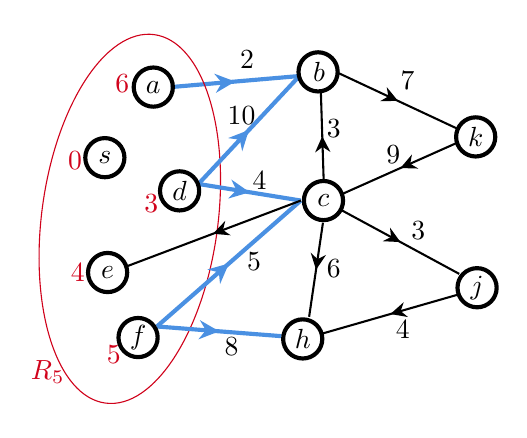
\begin{tikzpicture}[x=0.5pt,y=0.5pt,yscale=-1,xscale=1]
%uncomment if require: \path (0,296); %set diagram left start at 0, and has height of 296

%Straight Lines [id:da3320252336737717] 
\draw [color={rgb, 255:red, 74; green, 144; blue, 226 }  ,draw opacity=1 ][line width=1.5]    (119,48) -- (212,40) ;
\draw [shift={(165.5,44)}, rotate = 175.08] [fill={rgb, 255:red, 74; green, 144; blue, 226 }  ,fill opacity=1 ][line width=0.08]  [draw opacity=0] (14.56,-6.99) -- (0,0) -- (14.56,6.99) -- (9.67,0) -- cycle    ;
%Shape: Ellipse [id:dp2857420369455096] 
\draw  [color={rgb, 255:red, 208; green, 2; blue, 27 }  ,draw opacity=1 ] (26.24,134.88) .. controls (35.95,61.34) and (72.1,5.46) .. (106.98,10.07) .. controls (141.87,14.67) and (162.28,78.02) .. (152.57,151.56) .. controls (142.86,225.1) and (106.71,280.98) .. (71.83,276.37) .. controls (36.94,271.77) and (16.53,208.42) .. (26.24,134.88) -- cycle ;
%Straight Lines [id:da02943457575339692] 
\draw [color={rgb, 255:red, 74; green, 144; blue, 226 }  ,draw opacity=1 ][line width=1.5]    (139,118) -- (212,40) ;
\draw [shift={(175.5,79)}, rotate = 133.1] [fill={rgb, 255:red, 74; green, 144; blue, 226 }  ,fill opacity=1 ][line width=0.08]  [draw opacity=0] (14.56,-6.99) -- (0,0) -- (14.56,6.99) -- (9.67,0) -- cycle    ;
%Straight Lines [id:da7032022658079198] 
\draw [color={rgb, 255:red, 74; green, 144; blue, 226 }  ,draw opacity=1 ][line width=1.5]    (139,118) -- (213,130) ;
\draw [shift={(176,124)}, rotate = 189.21] [fill={rgb, 255:red, 74; green, 144; blue, 226 }  ,fill opacity=1 ][line width=0.08]  [draw opacity=0] (14.56,-6.99) -- (0,0) -- (14.56,6.99) -- (9.67,0) -- cycle    ;
%Straight Lines [id:da9416797747261806] 
\draw [color={rgb, 255:red, 74; green, 144; blue, 226 }  ,draw opacity=1 ][line width=1.5]    (109,221) -- (213,130) ;
\draw [shift={(161,175.5)}, rotate = 138.81] [fill={rgb, 255:red, 74; green, 144; blue, 226 }  ,fill opacity=1 ][line width=0.08]  [draw opacity=0] (14.56,-6.99) -- (0,0) -- (14.56,6.99) -- (9.67,0) -- cycle    ;
%Straight Lines [id:da6197316893700862] 
\draw [color={rgb, 255:red, 74; green, 144; blue, 226 }  ,draw opacity=1 ][line width=1.5]    (109,221) -- (199,228) ;
\draw [shift={(154,224.5)}, rotate = 184.45] [fill={rgb, 255:red, 74; green, 144; blue, 226 }  ,fill opacity=1 ][line width=0.08]  [draw opacity=0] (14.56,-6.99) -- (0,0) -- (14.56,6.99) -- (9.67,0) -- cycle    ;
%Straight Lines [id:da7705917014251779] 
\draw [color={rgb, 255:red, 0; green, 0; blue, 0 }  ,draw opacity=1 ][line width=0.75]    (86,178) -- (213,130) ;
\draw [shift={(149.5,154)}, rotate = 339.3] [fill={rgb, 255:red, 0; green, 0; blue, 0 }  ,fill opacity=1 ][line width=0.08]  [draw opacity=0] (11.61,-5.58) -- (0,0) -- (11.61,5.58) -- (7.71,0) -- cycle    ;
%Straight Lines [id:da7178806242260687] 
\draw [color={rgb, 255:red, 0; green, 0; blue, 0 }  ,draw opacity=1 ][line width=0.75]    (326,78) -- (240.5,38) ;
\draw [shift={(283.25,58)}, rotate = 205.07] [fill={rgb, 255:red, 0; green, 0; blue, 0 }  ,fill opacity=1 ][line width=0.08]  [draw opacity=0] (11.61,-5.58) -- (0,0) -- (11.61,5.58) -- (7.71,0) -- cycle    ;
%Straight Lines [id:da2873203830948724] 
\draw [color={rgb, 255:red, 0; green, 0; blue, 0 }  ,draw opacity=1 ][line width=0.75]    (326.5,88) -- (243.5,125) ;
\draw [shift={(285,106.5)}, rotate = 335.97] [fill={rgb, 255:red, 0; green, 0; blue, 0 }  ,fill opacity=1 ][line width=0.08]  [draw opacity=0] (11.61,-5.58) -- (0,0) -- (11.61,5.58) -- (7.71,0) -- cycle    ;
%Straight Lines [id:da9325647569597147] 
\draw [color={rgb, 255:red, 0; green, 0; blue, 0 }  ,draw opacity=1 ][line width=0.75]    (327.5,183) -- (242.5,137) ;
\draw [shift={(285,160)}, rotate = 208.42] [fill={rgb, 255:red, 0; green, 0; blue, 0 }  ,fill opacity=1 ][line width=0.08]  [draw opacity=0] (11.61,-5.58) -- (0,0) -- (11.61,5.58) -- (7.71,0) -- cycle    ;
%Straight Lines [id:da8240281406202591] 
\draw [color={rgb, 255:red, 0; green, 0; blue, 0 }  ,draw opacity=1 ][line width=0.75]    (219,214) -- (229,146) ;
\draw [shift={(224,180)}, rotate = 278.37] [fill={rgb, 255:red, 0; green, 0; blue, 0 }  ,fill opacity=1 ][line width=0.08]  [draw opacity=0] (11.61,-5.58) -- (0,0) -- (11.61,5.58) -- (7.71,0) -- cycle    ;
%Straight Lines [id:da6386544223700206] 
\draw [color={rgb, 255:red, 0; green, 0; blue, 0 }  ,draw opacity=1 ][line width=0.75]    (229,226) -- (326.5,198) ;
\draw [shift={(277.75,212)}, rotate = 343.98] [fill={rgb, 255:red, 0; green, 0; blue, 0 }  ,fill opacity=1 ][line width=0.08]  [draw opacity=0] (11.61,-5.58) -- (0,0) -- (11.61,5.58) -- (7.71,0) -- cycle    ;
%Straight Lines [id:da7268529078901531] 
\draw [color={rgb, 255:red, 0; green, 0; blue, 0 }  ,draw opacity=1 ][line width=0.75]    (229.5,115) -- (227.5,52) ;
\draw [shift={(228.5,83.5)}, rotate = 88.18] [fill={rgb, 255:red, 0; green, 0; blue, 0 }  ,fill opacity=1 ][line width=0.08]  [draw opacity=0] (11.61,-5.58) -- (0,0) -- (11.61,5.58) -- (7.71,0) -- cycle    ;

% Text Node
\draw (16,244) node [anchor=north west][inner sep=0.75pt]   [align=left] {$\displaystyle \textcolor[rgb]{0.82,0.01,0.11}{R}\textcolor[rgb]{0.82,0.01,0.11}{_{5}}$};
% Text Node
\draw (43,93) node [anchor=north west][inner sep=0.75pt]   [align=left] {$\displaystyle \textcolor[rgb]{0.82,0.01,0.11}{0}$};
% Text Node
\draw (167.24,20.06) node [anchor=north west][inner sep=0.75pt]   [align=left] {$\displaystyle 2$};
% Text Node
\draw  [line width=1.5]   (71.38, 99) circle [x radius= 14.15, y radius= 14.15]   ;
\draw (71.38,99) node   [align=left] {$\displaystyle s$};
% Text Node
\draw (77,37) node [anchor=north west][inner sep=0.75pt]   [align=left] {$\displaystyle \textcolor[rgb]{0.82,0.01,0.11}{6}$};
% Text Node
\draw  [line width=1.5]   (106.38, 48) circle [x radius= 14.15, y radius= 14.15]   ;
\draw (106.38,48) node   [align=left] {$\displaystyle a$};
% Text Node
\draw (98,124) node [anchor=north west][inner sep=0.75pt]   [align=left] {$\displaystyle \textcolor[rgb]{0.82,0.01,0.11}{3}$};
% Text Node
\draw  [line width=1.5]   (125.38, 123) circle [x radius= 14.15, y radius= 14.15]   ;
\draw (125.38,123) node   [align=left] {$\displaystyle d$};
% Text Node
\draw (45,174) node [anchor=north west][inner sep=0.75pt]   [align=left] {$\displaystyle \textcolor[rgb]{0.82,0.01,0.11}{4}$};
% Text Node
\draw  [line width=1.5]   (73.38, 182) circle [x radius= 14.15, y radius= 14.15]   ;
\draw (73.38,182) node   [align=left] {$\displaystyle e$};
% Text Node
\draw  [line width=1.5]   (225.48, 37) circle [x radius= 14.15, y radius= 14.15]   ;
\draw (219.98,37) node [anchor=west] [inner sep=0.75pt]   [align=left] {$\displaystyle b$};
% Text Node
\draw  [line width=1.5]   (229.38, 130) circle [x radius= 14.15, y radius= 14.15]   ;
\draw (229.38,130) node   [align=left] {$\displaystyle c$};
% Text Node
\draw  [line width=1.5]   (339.38, 84) circle [x radius= 14.15, y radius= 14.15]   ;
\draw (339.38,84) node   [align=left] {$\displaystyle k$};
% Text Node
\draw  [line width=1.5]   (214.38, 230) circle [x radius= 14.15, y radius= 14.15]   ;
\draw (214.38,230) node   [align=left] {$\displaystyle h$};
% Text Node
\draw (71,233) node [anchor=north west][inner sep=0.75pt]   [align=left] {$\displaystyle \textcolor[rgb]{0.82,0.01,0.11}{5}$};
% Text Node
\draw  [line width=1.5]   (95.38, 229) circle [x radius= 14.15, y radius= 14.15]   ;
\draw (95.38,229) node   [align=left] {$\displaystyle f$};
% Text Node
\draw  [line width=1.5]   (340.38, 193) circle [x radius= 14.15, y radius= 14.15]   ;
\draw (340.38,193) node   [align=left] {$\displaystyle j$};
% Text Node
\draw (158.24,60.06) node [anchor=north west][inner sep=0.75pt]   [align=left] {$\displaystyle 10$};
% Text Node
\draw (176.24,107.06) node [anchor=north west][inner sep=0.75pt]   [align=left] {$\displaystyle 4$};
% Text Node
\draw (172.24,166.06) node [anchor=north west][inner sep=0.75pt]   [align=left] {$\displaystyle 5$};
% Text Node
\draw (156,227.5) node [anchor=north west][inner sep=0.75pt]   [align=left] {$\displaystyle 8$};
% Text Node
\draw (283.24,35.06) node [anchor=north west][inner sep=0.75pt]   [align=left] {$\displaystyle 7$};
% Text Node
\draw (291,143) node [anchor=north west][inner sep=0.75pt]   [align=left] {$\displaystyle 3$};
% Text Node
\draw (279.75,215) node [anchor=north west][inner sep=0.75pt]   [align=left] {$\displaystyle 4$};
% Text Node
\draw (273,88.47) node [anchor=north west][inner sep=0.75pt]   [align=left] {$\displaystyle 9$};
% Text Node
\draw (230,70) node [anchor=north west][inner sep=0.75pt]   [align=left] {$\displaystyle 3$};
% Text Node
\draw (230,171) node [anchor=north west][inner sep=0.75pt]   [align=left] {$\displaystyle 6$};


\end{tikzpicture}

}
%%% \caption{
%%% Assume that we already know $R_5 = (s, d, e, f, a)$; the distance to each vertex in $R_5$ is marked in red.
%%% Try above formulas in Figure~\ref{fig:extension}.
%%% Answer: $dist_5(b) = \min\{6 + 2, 3 + 10\} = 8$, $dist_5(c) = \min\{3 + 4,  5 + 5\} = 7$, $dist_5(h) = 5 + 8 = 13$, 
%%% $dist_5(k) = \infty$, $dist_5(j) = \infty$;
%%% hence $v_6^* = c$ and $distance(s,v_6^*) = dist_5(c) = 7$.}
%%% \label{fig:extension2}
%%% \end{figure}

The reason we introduce $dist_k$ is that, $dist_{k+1}$ can be calculated 
in an incremental way by largely reusing $dist_k$.
This is much more efficiently than directly calculating $dist_{k+1}$ using the definition. 
To see the details, recall its definition, for any $v\in V\setminus R_{k+1}$, we have 
$$dist_{k+1}(v) = \textstyle \min_{u\in R_{k+1}, (u, v)\in E} (distance(s, u) + l(u,v)).$$
Note that $R_{k+1} = R_k \cup \{v_{k+1}^*\}$. Hence
\begin{displaymath}
dist_{k+1}(v) = \left\{
\begin{array}{llllll}
\min\{ dist_k(v), distance(s, v_{k+1}^*) + l(v_{k+1}^*, v) \} & \textrm{ if } (v_{k+1}^*, v) \in E \\
dist_k(v) & \textrm{ if } (v_{k+1}^*, v) \not\in E
\end{array}
\right.
\end{displaymath}

In other words, when calculating $dist_{k+1}$, we only need to examine the out-edges of $v_{k+1}^*$
and update only if the use of $v_{k+1}^*$ leads to a shorter path. The pseudo-code of
calculating $dist_{k+1}$ from $dist_k$ is given below.
Before calling this updating procedure, we assume $dist_{k+1}$ is initialized as $dist_k$;
that is the update-dist procedure below just update for vertices whose dist values might be reduced.
(In the complete algorithm, you will see that we will use one $dist$ array for all $k$, hence such initialization is not necessary.)

\begin{minipage}{0.8\textwidth}
	\aaA {6}{procedure update-dist~($v_{k+1}^*$)}\xxx
	\aaB {4}{for $(v_{k+1}^*, v) \in E$}\xxx
	\aaC {2}{if~($dist_k(v_{k+1}^*) + l(v_{k+1}^*, v) < dist_{k+1}(v) $)}\xxx
	\aad {$dist_{k+1}(v) = dist_k(v_{k+1}^*) + l(v_{k+1}^*, v)$;}\xxx
	\aac {end if;}\xxx
	\aab {end for;}\xxx
	\aaa {end procedure;}\xxx
\end{minipage}

Try above procedure with the example below.

\begin{figure}[h!]
\centering{

\tikzset{every picture/.style={line width=0.75pt}} %set default line width to 0.75pt        

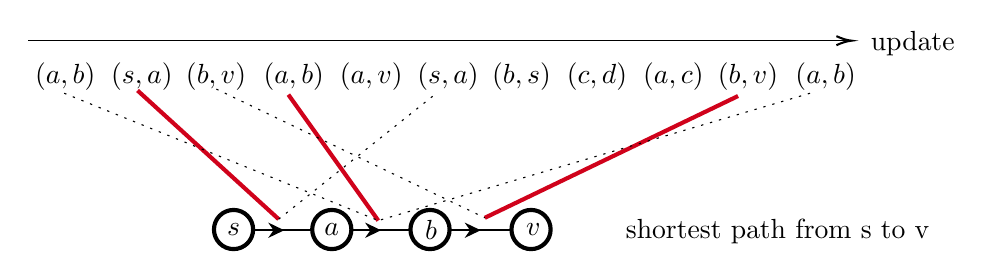
\begin{tikzpicture}[x=0.5pt,y=0.5pt,yscale=-1,xscale=1]
%uncomment if require: \path (0,193); %set diagram left start at 0, and has height of 193

%Straight Lines [id:da42563372855460047] 
\draw [color={rgb, 255:red, 0; green, 0; blue, 0 }  ,draw opacity=1 ][line width=0.75]    (253.5,160) -- (296.5,160) ;
\draw [shift={(275,160)}, rotate = 180] [fill={rgb, 255:red, 0; green, 0; blue, 0 }  ,fill opacity=1 ][line width=0.08]  [draw opacity=0] (11.61,-5.58) -- (0,0) -- (11.61,5.58) -- (7.71,0) -- cycle    ;
%Straight Lines [id:da13574797376852343] 
\draw [color={rgb, 255:red, 0; green, 0; blue, 0 }  ,draw opacity=1 ][line width=0.75]    (325.5,160) -- (368.5,160) ;
\draw [shift={(347,160)}, rotate = 180] [fill={rgb, 255:red, 0; green, 0; blue, 0 }  ,fill opacity=1 ][line width=0.08]  [draw opacity=0] (11.61,-5.58) -- (0,0) -- (11.61,5.58) -- (7.71,0) -- cycle    ;
%Straight Lines [id:da9930965641121888] 
\draw    (20,23) -- (613,23) ;
\draw [shift={(615,23)}, rotate = 180] [color={rgb, 255:red, 0; green, 0; blue, 0 }  ][line width=0.75]    (10.93,-3.29) .. controls (6.95,-1.4) and (3.31,-0.3) .. (0,0) .. controls (3.31,0.3) and (6.95,1.4) .. (10.93,3.29)   ;
%Straight Lines [id:da09874107164515367] 
\draw [color={rgb, 255:red, 0; green, 0; blue, 0 }  ,draw opacity=1 ][line width=0.75]    (183.5,160) -- (226.5,160) ;
\draw [shift={(205,160)}, rotate = 180] [fill={rgb, 255:red, 0; green, 0; blue, 0 }  ,fill opacity=1 ][line width=0.08]  [draw opacity=0] (11.61,-5.58) -- (0,0) -- (11.61,5.58) -- (7.71,0) -- cycle    ;
%Straight Lines [id:da6519777460675502] 
\draw [color={rgb, 255:red, 208; green, 2; blue, 27 }  ,draw opacity=1 ][line width=1.5]    (201,152) -- (99,59) ;
%Straight Lines [id:da29298485524387174] 
\draw [color={rgb, 255:red, 208; green, 2; blue, 27 }  ,draw opacity=1 ][line width=1.5]    (273,153) -- (208,62) ;
%Straight Lines [id:da3208602618624562] 
\draw [color={rgb, 255:red, 208; green, 2; blue, 27 }  ,draw opacity=1 ][line width=1.5]    (350,151) -- (533,63) ;
%Straight Lines [id:da419202195721033] 
\draw  [dash pattern={on 0.84pt off 2.51pt}]  (46,61) -- (273,153) ;
%Straight Lines [id:da11015742569478726] 
\draw  [dash pattern={on 0.84pt off 2.51pt}]  (585,61) -- (273,153) ;
%Straight Lines [id:da5872263776878417] 
\draw  [dash pattern={on 0.84pt off 2.51pt}]  (201,152) -- (315,61) ;
%Straight Lines [id:da26779689112701766] 
\draw  [dash pattern={on 0.84pt off 2.51pt}]  (156,58) -- (350,151) ;

% Text Node
\draw  [line width=1.5]   (168.38, 159.47) circle [x radius= 14.15, y radius= 14.15]   ;
\draw (168.38,159.47) node   [align=left] {$\displaystyle s$};
% Text Node
\draw  [line width=1.5]   (239.38, 159.47) circle [x radius= 14.15, y radius= 14.15]   ;
\draw (239.38,159.47) node   [align=left] {$\displaystyle a$};
% Text Node
\draw  [line width=1.5]   (310.38, 159.47) circle [x radius= 14.15, y radius= 14.15]   ;
\draw (304.88,159.47) node [anchor=west] [inner sep=0.75pt]   [align=left] {$\displaystyle b$};
% Text Node
\draw  [line width=1.5]   (383.38, 159.47) circle [x radius= 14.15, y radius= 14.15]   ;
\draw (377.88,159.47) node [anchor=west] [inner sep=0.75pt]   [align=left] {$\displaystyle v$};
% Text Node
\draw (78.06,37) node [anchor=north west][inner sep=0.75pt]   [align=left] {$\displaystyle ( s,a)$};
% Text Node
\draw (572.6,37) node [anchor=north west][inner sep=0.75pt]   [align=left] {$\displaystyle ( a,b)$};
% Text Node
\draw (243.24,37) node [anchor=north west][inner sep=0.75pt]   [align=left] {$\displaystyle ( a,v)$};
% Text Node
\draw (132.12,37) node [anchor=north west][inner sep=0.75pt]   [align=left] {$\displaystyle ( b,v)$};
% Text Node
\draw (188.18,37) node [anchor=north west][inner sep=0.75pt]   [align=left] {$\displaystyle ( a,b)$};
% Text Node
\draw (407.42,37) node [anchor=north west][inner sep=0.75pt]   [align=left] {$\displaystyle ( c,d)$};
% Text Node
\draw (462.48,37) node [anchor=north west][inner sep=0.75pt]   [align=left] {$\displaystyle ( a,c)$};
% Text Node
\draw (299.3,37) node [anchor=north west][inner sep=0.75pt]   [align=left] {$\displaystyle ( s,a)$};
% Text Node
\draw (353.36,37) node [anchor=north west][inner sep=0.75pt]   [align=left] {$\displaystyle ( b,s)$};
% Text Node
\draw (627,14) node [anchor=north west][inner sep=0.75pt]   [align=left] {update};
% Text Node
\draw (23,37) node [anchor=north west][inner sep=0.75pt]   [align=left] {$\displaystyle ( a,b)$};
% Text Node
\draw (516.54,37) node [anchor=north west][inner sep=0.75pt]   [align=left] {$\displaystyle ( b,v)$};
% Text Node
\draw (450,150) node [anchor=north west][inner sep=0.75pt]   [align=left] {shortest path from s to v};


\end{tikzpicture}

}
\caption{Following Figure~\ref{fig:extension2}, we have that $v_6^* = c$.
We now want to calculate $dist_6$ using $dist_5$. We consider the out-edges of $c$, marked as thick blue edges.
We have, 
$dist_6(b) = \min\{dist_5(b), 7 + 3\}= \min\{8, 10\} = 8$, 
$dist_6(h) = \min\{dist_5(h), 7 + 6\}= \min\{13, 13\} = 13$, 
$dist_6(k) = dist_5(k) = \infty$, 
$dist_6(j) = \min\{dist_5(j), 7 + 3\}= \min\{\infty, 10\} = 10$.  }
\label{fig:update}
\end{figure}

%The above procedure enables fast calculation of $dist_k$.
The last piece of Dijkstra's algorithm comes with the use of \emph{priority queue}
to quickly pick the next closest vertex, i.e., to calculate $v_{k+1}^* = \arg\min_{v\in V\setminus R_k} dist_k(v)$.
To this end, the priority queue $PQ$ always stores $V\setminus R_k$,
and for each vertex $v$ that is stored in $PQ$, its priority is $dist_k(v)$.
In this way, every time we call find-min~($PQ$), it gives us $\min_{v\in V\setminus R_k} dist_k(v)$.

The pseudo-code for complete Dijkstra's algorithm is given below.
First, instead of maintaining a $dist_k$ array for each separate $k$, we just need 
to maintain a single $dist$ array~(the index $k$ will increase implicitly when the next closest vertex
gets identified and removed from the priority-queue). 
Second, we do not need to implicitly maintain $R_k$,
as $PQ$ is always complement to $R_k$.
In order to maintain this invariant, we delete the next closed vertex $u$, 
by calling delete-min, at the time of identifying $u$.
In the update-list procedure, in order to guarantee that the priority of $v$ is
always $dist(v)$, we call decrease-key every time we update $dist(v)$.

%We use array $dist$ of size $|V|$ to store $dist_k$.

Recall that Dijkstra's algorithm sequentially identifies the closests vertices from $s$.
Formally, if $u$ is removed from $PQ$ before $v$, then $distance(s, u) \le distance(s, v)$.

Where are the final distances from $s$?  They are in array $dist$.
This is because, at the time a vertex $u$ is picked by find-min and 
removed from $PQ$,
$dist$ value for this vertex $u$ is exactly its distance, i.e., $dist(u) = distance(s, u)$.
This dist value for $u$ will remain unchanged till the end of the algorithm.
Notice though, later in the algorithm, when $v$ is picked by find-min~(and removed from $PQ$),
there might be an edge $(v, u)$ and therefore $dist(v) + l(v, u)$ will be compared with $dist(u)$ according to the algorithm,
and if the former is smaller than the later, $dist(u)$ will be reduced/changed.
(See an example in Figure~2, edge~$(c, e)$.)
But such change will never happen. This is because, $u$ is picked before $v$, implying that
$distance(s, u) \le distance(s, v)$. Hence $dist(v) + l(v, u) = distance(s, v) + l(v, u) > distance(s, v) \ge distance(s, u) = dist(u)$.
So, the update to $dist(u)$ will not happen.

Another way to understand why such update to $dist(u)$ will not happen
is that $dist(u)$ is always an upper bound of $distance(s,u)$.
When $u$ gets removed from $PQ$, this bound is reached, i.e., $dist(u) = distance(s, u)$.
Hence after that $dist(u)$ will remain this minimized value and hence cannot get further reduced.

\begin{minipage}{0.8\textwidth}
	\aaA {16}{Algorithm Dijkstra~($G = (V, E)$, $l(e)$ for any $e\in E$, $s \in V$)}\xxx
	\aab {$dist[v] = \infty$, for any $v\in V$;}\xxx
	\aab {init an empty priority queue $PQ$;}\xxx
	\aab {for any $v\in V$: insert~($PQ$, $v$), where the priority of $v$ is $\infty$;}\xxx
	\aab {$dist[s] = 0$;}\xxx
	\aab {decrease-key~($PQ, s, 0$);}\xxx
	\aaB {9}{while~(empty~($PQ$) = false)}\xxx
	\aac {$u$ = find-min~($PQ$);}\xxx
	\aac {delete-min~($PQ$);}\xxx
	\aaC {5}{for each edge~$(u, v)\in E$}\xxx
	\aaD {3}{if~($dist[v] > dist[u] + l(u,v)$)}\xxx
	\aae {$dist[v] = dist[u] + l(u,v)$;}\xxx
	\aae {decrease-key~($PQ$, $v$, $dist[v]$);}\xxx
	\aad {end if;}\xxx
	\aac {end for;}\xxx
	\aab {end while;}\xxx
	\aaa {end algorithm;}\xxx
\end{minipage}


The running time of Dijkstra's algorithmd depends on the specific implementation of priority queue used.
Consider using binary heap. The break-down of running time is given below.
Note that each vertex will be picked from the $PQ$ at most once and each edge will be examined at most once~(for directed graph) or at most twice~(for undirected graph).
The total running time is $O((|V|+|E|)\log |V|)$.
\vspace*{-\topsep}
\begin{enumerate}
\item initialization: $\Theta(|V|)$;
\item insert~($PQ$): $|V| \times O(\log |V|)$;
\item empty~($PQ$): $|V| \times \Theta(1)$;
\item find-min~($PQ$): $|V| \times \Theta(1)$;
\item delete-min~($PQ$): $|V| \times O(\log |V|)$;
\item updating-dist: $|E| \times \Theta(1)$;
\item decrease-key~($PQ$): $|E| \times O(\log |V|)$;
\end{enumerate}

